\documentclass{article}
\usepackage{amsfonts, amsthm, amsmath, amssymb, mathtools, ulem, mathrsfs, physics, esint, siunitx, tikz-cd}
\usepackage{pdfpages, fullpage, color, microtype, cancel, textcomp, markdown, hyperref, graphicx}
\usepackage{enumitem}
\graphicspath{{./images/}}
\usepackage[english]{babel}
\usepackage[autostyle, english=american]{csquotes}
\MakeOuterQuote{"}
\usepackage{xparse}
\usepackage{tikz}
\usepackage{algpseudocode}

% fonts
\def\mbb#1{\mathbb{#1}}
\def\mfk#1{\mathfrak{#1}}
\def\mbf#1{\mathbf{#1}}
\def\tbf#1{\textbf{#1}}

% common bold letters
\def\bP{\mbb{P}}
\def\bC{\mbb{C}}
\def\bH{\mbb{H}}
\def\bI{\mbb{I}}
\def\bR{\mbb{R}}
\def\bQ{\mbb{Q}}
\def\bZ{\mbb{Z}}
\def\bN{\mbb{N}}

% brackets
\newcommand{\br}[1]{\left(#1\right)}
\newcommand{\sbr}[1]{\left[#1\right]}
\newcommand{\brc}[1]{\left\{#1\right\}}
\newcommand{\lbr}[1]{\left\langle#1\right\rangle}

% matrices
\newcommand{\m}[2][b]{\begin{#1matrix}#2\end{#1matrix}}
\newcommand{\arr}[3][\sbr]{#1{\begin{array}{#2}#3\end{array}}}

% misc
\NewDocumentCommand{\app}{O{x} O{\infty}}{\xrightarrow{#1\to#2}}
\renewcommand{\ss}{\subset}
\newcommand{\vn}{\varnothing}
\newcommand{\inv}{^{-1}}
\newcommand{\imp}{\implies}
\newcommand{\impleft}{\reflectbox{$\implies$}}
\renewcommand{\bar}{\overline}
\renewcommand{\d}{\partial}
\newcommand{\pf}{\tbf{Proof. }}

% greek
\newcommand{\e}{\epsilon}
\newcommand{\p}{\varphi}
\renewcommand{\t}{\theta}
\renewcommand{\a}{\alpha}
\renewcommand{\b}{\beta}
\newcommand{\K}{\mathcal{K}}
\renewcommand{\l}{\lambda}

% title
\title{Scientific Computing HW 8}
\author{Ryan Chen}
%\date{\today}
\setlength{\parindent}{0pt}


\begin{document}
	
\maketitle



\begin{enumerate}
	
	
	
	\item To show that the algorithms are equivalent, we rewrite $\a_k,r_{k+1},\b_{k+1}$. Rewrite $\a_k$ as
	\begin{align*}
		\a_k &= -\frac{r_k^Tp_k}{p_k^TAp_k} \\
		&= -\frac{r_k^T(-r_k+\b_kp_{k-1})}{p_k^TAp_k} & p_k = -r_k+\b_kp_{k-1} \\
		&= \frac{r_k^Tr_k}{p_k^TAp_k} & \text{$r_k^Tp_{k-1}=0$ by Theorem 5.2 in [NW]}
	\end{align*}
	Rewrite $r_{k+1}$ as
	\begin{align*}
		r_{k+1} &= Ax_{k+1} - b \\
		&= A(x_k+\a_kp_k) - b \\
		&= Ax_k - b + \a_kAp_k \\
		&= r_k + \a_kAp_k
	\end{align*}
	The expressions for $\a_k,r_{k+1}$ give
	\[Ap_k = \frac{r_{k+1}-r_k}{\a_k} = \frac{p_k^TAp_k(r_{k+1}-r_k)}{r_k^Tr_k}\]
	Use this to rewrite $\b_{k+1}$ as
	\begin{align*}
		\b_{k+1} &= \frac{r_{k+1}^TAp_k}{p_k^TAp_k} \\
		&= \frac{r_{k+1}^T(r_{k+1}-r_k)}{r_k^Tr_k} \\
		&= \frac{r_{k+1}^Tr_{k+1}}{r_k^Tr_k} & \text{$r_{k+1}^Tr_k=0$ by Theorem 5.3 in [NW]}
	\end{align*}
	
	
	
	\pagebreak
	
	
	
	\item As a preliminary, define the Krylov subspaces (the first definition is a natural extension to $k=0$)
	\[\K_0 := \brc0,
	\quad \K_k = \K(A,r,k) := \mathrm{span}\brc{A^ir: 0\le i\le k-1},~ k\ge1\]
	
	
	We will divide the proof into the following claims:
	\begin{itemize}
		
		
		\item Claim 1: We can define the greatest integer $k'$ such that $\dim\K_{k'}=k'$.
		
		Observe that $\dim\K_0=\dim\brc0=0$. Also observe that $A$ has $n$ rows, so that for all $k'$ we have that $\K_{k'}$ is a subspace of $\bR^n$ hence $\dim\K_{k'}\le n$. Thus there is a nonzero finite number of integers $k'$ satisfying $\dim\K_{k'}=k'$, so that we can pick $k'$ to be the greatest such integer. 
		
		
		\item Claim 2: $\K_p=\K_{k'}$ for all $p\ge k'+1$. We will prove this by induction.
		
		Base case $p=k'+1$: We have $\dim\K_{k'+1}\le k'+1$, and by Claim 1 we have $\dim\K_{k'+1}\ne k'+1$, hence
		\[\dim\K_{k'+1}<k'+1
		\imp \dim\K_{k'+1}\le k'
		\imp \dim\K_{k'+1}\le\dim\K_{k'}\]
		Since $\K_{k'}$ is a subspace of $\K_{k'+1}$, we have $\dim\K_{k'}\le\dim\K_{k'+1}$. Thus $\dim\K_{k'}=\dim\K_{k'+1}$, and using again the fact $\K_{k'}$ is a subspace of $\K_{k'+1}$, we have $\K_{k'}=\K_{k'+1}$.
		
		Inductive step: Fix $p\ge k'+1$ and assume $\K_p=\K_{k'}$. This gives
		\[A^ir\in\K_{k'},~ 0\le i\le p-1 \quad (2.1)\]
		It remains to show $A^pr\in\K_{k'}$ so that we can conclude $\K_{p+1}=\K_{k'}$. Setting $i=p-1$ in (2.1) gives $A^{p-1}r\in\K_{k'}$, so $A^{p-1}r=\sum_{i=0}^{k'-1}c_iA^ir$ for some scalars $c_i$. Then
		\[A^pr = \sum_{i=0}^{k'-1} c_iA^{i+1}r
		= \sum_{i=1}^{k'} c_{i-1}A^ir
		= \sum_{i=1}^{k'-1} c_{i-1}A^ir + c_{k'-1}A^{k'}r\]
		The RHS sum over $i$ is in $\K_{k'}$ by definition of $\K_{k'}$, and the last RHS term is in $\K_{k'}$ by setting $i=k'$ in (2.1), thus $A^pr\in\K_{k'}$.
		
		
		\item Claim 3: If $r=By$ for some $y\in\bR^k$ then $k=k'$. We conclude that $\K_p=\K_k$ for all $p\ge k+1$.
		
		We aim to show that $k'\le k$ and $k'\ge k$. To show that $k'\le k$, consider that for all $i\ge0$,
		\[A^ir = A^iBy = BC^iy \in \mathrm{col}B\]
		Thus $\K_{k'}$ is a subspace of $\mathrm{col}B$. This along with $\rank B=k$ and Claim 1 gives $k'\le k$.
		
		To show that $k'\ge k$, suppose for the sake of contradiction that $k'<k$. This along with Claim 2 gives $\K_k=\K_{k'}$, hence $\dim\K_k=k'$. This means that $A^ir,~0\le i\le k-1$ are linearly dependent, so there exist scalars $\a_i$, not all zero, such that $\sum_{i=0}^{k-1}\a_i A^ir=0$. Let $B$ have columns $b_j,~1\le j\le k$ and rewrite the LHS,
		\[\sum_{i=0}^{k-1} \a_i A^ir = \sum_{i=0}^{k-1}B\underbrace{\a_iC^iy}_{=:z_i}
		= \sum_{i=0}^{k-1} Bz_i
		= \sum_{i=0}^{k-1}\sum_{j=1}^k z_{ij}b_j
		= \sum_{j=1}^k\sbr{\sum_{i=0}^{k-1}z_{ij}}b_j\]
		Since the $b_j$'s are linearly independent,
		\[\sum_{i=0}^{k-1}z_{ij} = 0,~ 1\le j\le k \quad (2.2)\]
		The LHS of (2.2) is a multivariate polynomial in terms of the entries of $C$ that is nonzero (the $\a_i$'s are not all zero) and has degree at most $k-1$. But (2.2) implies that it has at least $k$ distinct roots, so its degree is at least $k$, a contradiction. We conclude that $k'\ge k$.
		
		
	\end{itemize}
	
	
	
	\pagebreak
	
	
	
	\item
	
	\begin{enumerate}
		
		
		
		\item Define $Q\in\mathcal P_{k+1}$ by
		\[Q(\l) := C\sbr{\frac12(\l_1+\l_{n-k})-\l}\prod_{i=n-k+1}^{n}(\l_{i}-\l)\]
		To find $C$ we impose $Q(0)=1$.
		\[1 = Q(0) = \frac{C}{2}(\l_1+\l_{n-k})\prod_{i=n-k+1}^{n}\l_{i}
		\imp C = \frac{1}{\frac12(\l_1+\l_{n-k})}\prod_{i=n-k+1}^{n}\frac{1}{\l_{i}}\]
		Hence
		\[Q(\l) = \frac{\frac12(\l_1+\l_{n-k})-\l}{\frac12(\l_1+\l_{n-k})}\prod_{i=n-k+1}^n \br{1-\frac{\l}{\l_i}}\]
		
		
		
		\item Factor theorem: Given $R\in\mathcal P_k$, we have $R(\l)=(\l-\l_0)P(\l)$ for some $P\in\mathcal P_{k-1}$ iff $R(\l_0)=0$.
		
		From $Q(0)-1=0$ and the theorem, $Q(\l)-1=\l P(\l)$ for some $P\in\mathcal P_k$, hence $P(\l)=\frac{Q(\l)-1}{\l}$.
		
		
		
		\item Using $P\in\mathcal P_k$ from part (b),
		\[\min_{P_k\in\mathcal P_k}\max_{1\le i\le n}[1+\l_iP_k(\l_i)]^2
		\le \max_{1\le i\le n}[1+\l_iP(\l_i)]^2
		= \max_{1\le i\le n}Q^2(\l_i)\]
		Plug this into the ansatz to get
		\[\norm{x_{k+1}-x^*}_A^2 \le \max_{1\le i\le n}Q^2(\l_i)\norm{x_0-x^*}_A^2\]
		
		
		
		\item From part (a),
		\[Q^2(\l) = \br{\frac{\l-\frac12(\l_1+\l_{n-k})}{\frac12(\l_1+\l_{n-k})}}^2\prod_{i=n-k+1}^n \br{1-\frac{\l}{\l_i}}^2\]
		We have $Q^2(\l_i) = 0$ for $n-k+1\le i\le n$, and the assumption $\l_1\le\l_2\le\dots\le\l_n$ gives
		\[Q^2(\l_i) \le \br{\frac{\l-\frac12(\l_1+\l_{n-k})}{\frac12(\l_1+\l_{n-k})}}^2,~ 1\le i\le n-k\]
		Together, these computations give
		\[\max_{1\le i\le n} Q^2(\l_i) \le \max_{1\le i\le n-k} \br{\frac{\l_i-\frac12(\l_1+\l_{n-k})}{\frac12(\l_1+\l_{n-k})}}^2
		\le \max_{\l\in[\l_1,\l_{n-k}]}\br{\frac{\l-\frac12(\l_1+\l_{n-k})}{\frac12(\l_1+\l_{n-k})}}^2\]
		This along with the result of part (c) gives
		\[\norm{x_{k+1}-x^*}_A^2 \le \max_{\l\in[\l_1,\l_{n-k}]}\br{\frac{\l-\frac12(\l_1+\l_{n-k})}{\frac12(\l_1+\l_{n-k})}}^2 \norm{x_0-x^*}_A^2\]
		
		
		
		\item The function
		\[f(\l) := \br{\frac{\l-a}{a}}^2,
		\quad a := \frac12(\l_1+\l_{n-k})\]
		is a concave up parabola which is even wrt $\l=a$. With $a$ being the midpoint between $\l_1$ and $\l_{n-k}$, we see that $f$ attains its maximum on the interval $[\l_1,\l_{n-k}]$ at the endpoints $\l_1$ and $\l_{n-k}$.
		\[\max_{\l\in[\l_1,\l_{n-k}]} f(\l) = f(\l_1) = \br{\frac{\l_{n-k}-\l_1}{\l_{n-k}+\l_1}}^2\]
		
		
		
		\item From parts (d) and (e),
		\[\norm{x_{k+1}-x^*}_A^2 \le \br{\max_{\l\in[\l_1,\l_{n-k}]} f(\l)}\norm{x_0-x^*}_A^2
		= \br{\frac{\l_{n-k}-\l_1}{\l_{n-k}+\l_1}}^2\norm{x_0-x^*}_A^2\]
		
		
		
	\end{enumerate}



	\pagebreak
	
	
	
	\item Code: \url{https://github.com/RokettoJanpu/scientific-computing-1-redux/blob/main/hw8/hw8.ipynb}
	
	\begin{center}
		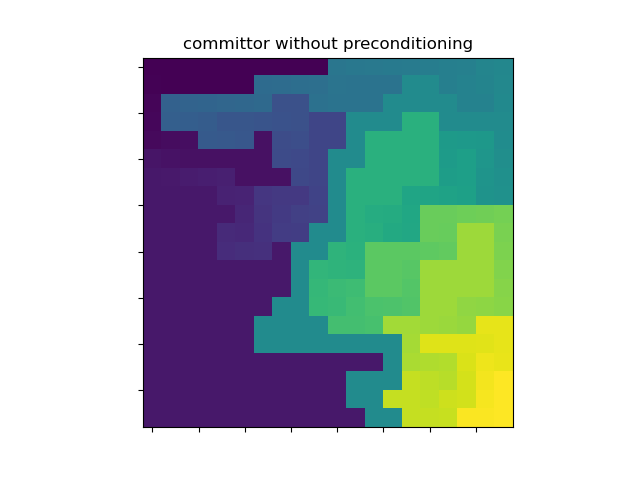
\includegraphics[scale=.4]{committor without preconditioning}
		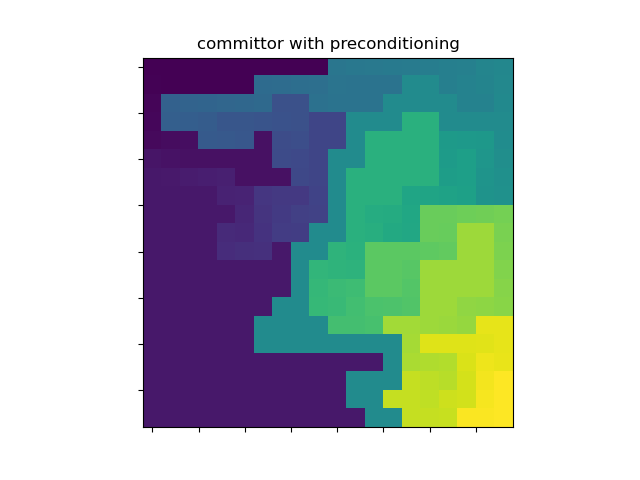
\includegraphics[scale=.4]{committor with preconditioning}
		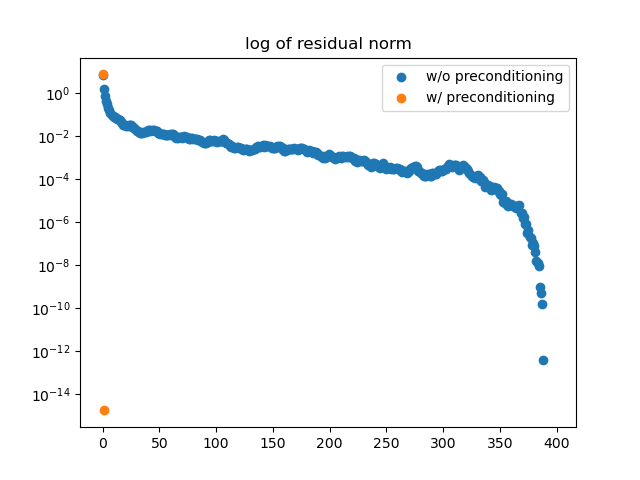
\includegraphics[scale=.5]{residual norm}
	\end{center}
	CG with conditioning only took one iteration, resulting in only two plotted points.
	
	
	
\end{enumerate}
	
	
	
	
\end{document}